\chapter{Introduction}
\section{Water Cycle}
Water is one of the most important ingredient of life; it regulates climate and many industeries need water as coolant, solvent,rea material, etc. Water covers about 71\% of the earth's surface. However, 96.5 \%of the water on the earth is in the oceans, 1.7\% is in ice caps, which means only 1.4 \% is the fresh water on land \cite{gleick1993water}. The water on earth is variable depending on a wide range of climatic variables. A very little variability of the hydrology cycle can have big effects on water resources. \cite{evans1996effects}\\\\
The hydrology cycle (see figure \ref{fig:hydrologic cycle}) includes 3 major compartments: evaporation, precipitation and runoff. The water evaporates from the oceans and the land surface as vapor to become part of the atmosphere along with water from evapotranspiration, which is water transpired from plants and evaporated from the soil and the cooler temperature causes the vapor into clouds. The clouds fall out of the sky as precipitation, which includes rain, snow and ice. Most precipitation falls back into the oceans or onto land. Precipitated water may be intercepted by vegetation, become overland flow over the ground surface, flow through the soil as subsurface flow and discharge into streams as surface runoff. The process can be simplified as:
\begin{equation}
	 Pre - ET - R = \frac{dS}{dt}
\end{equation}
where
\begin{table}[htbp]
	\begin{tabular}{ll}
		$Pre$   & Precipitation    \\ 
		$ET$    & Evatranspiration \\ \
		$R$     & Surface Runoff \\ 
		$dS / dt$ & total water storage change \\ 
	\end{tabular}
\end{table}
\begin{figure}[htbp]
	\centering
	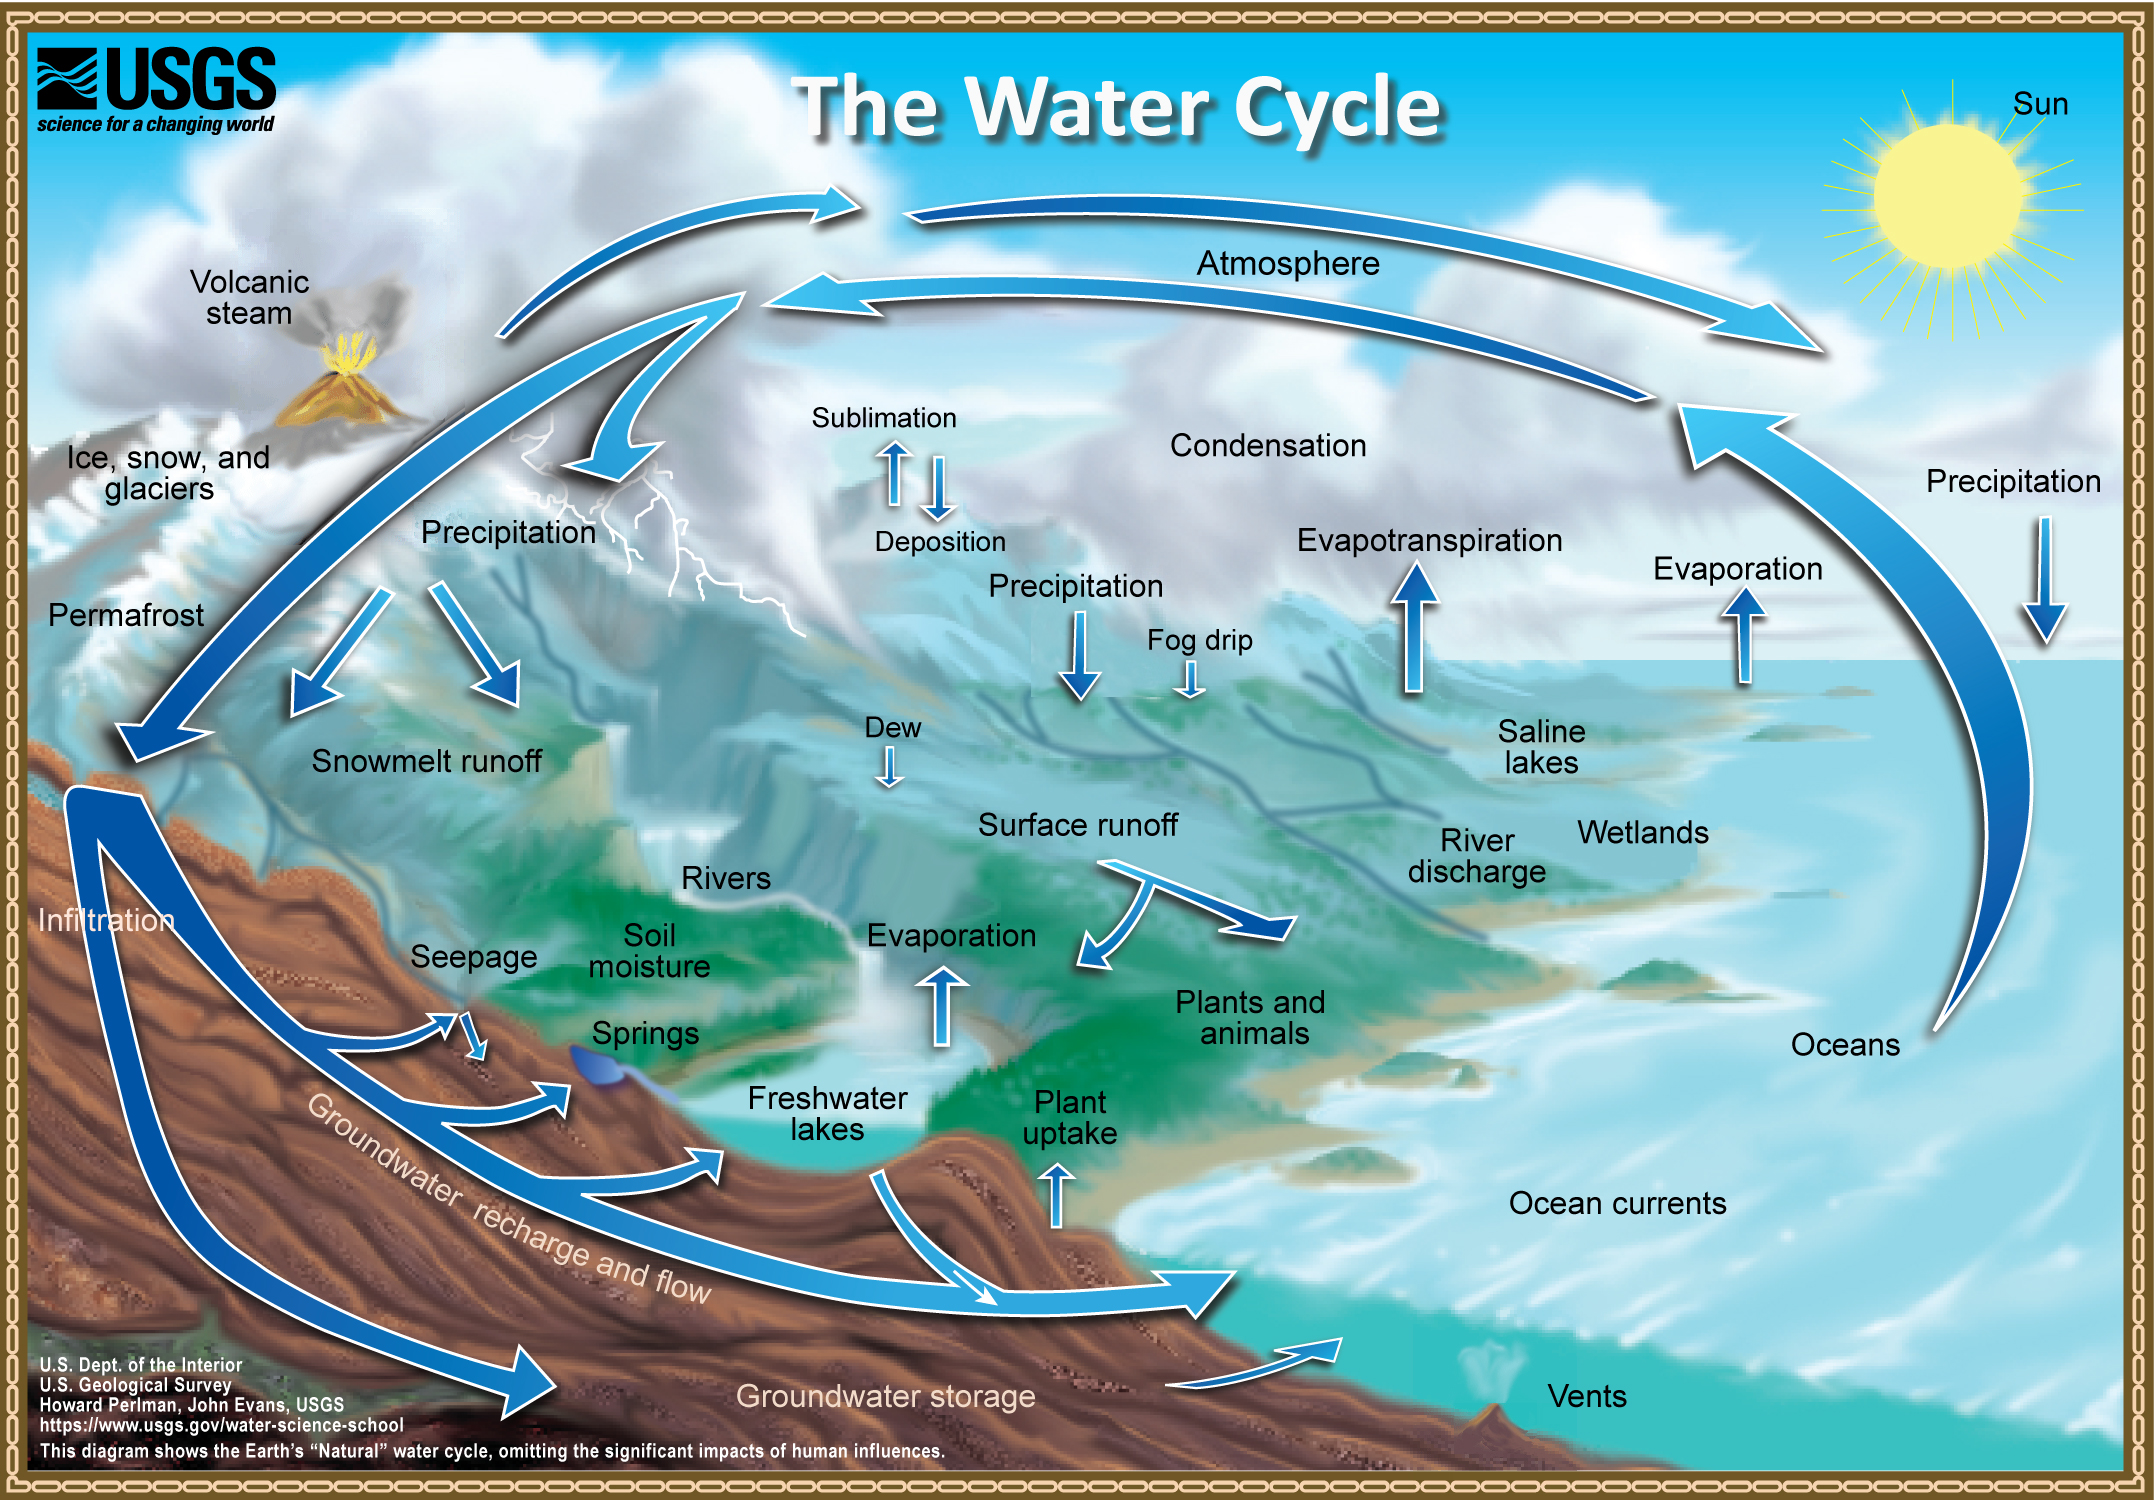
\includegraphics[width=0.7\textwidth]{water-cycle-natural} % Datei in "bilder/" bei LaTeX: eps, bei PDFLaTeX: jpg (o.ä.) 
	\caption{hydrologic cycle} 
	\label{fig:hydrologic cycle}
\end{figure}
\subsection{Precipitation}
Precipitation is any form of water particle, solid or liquid, that falls from the atmosphere and reaches the ground. Precipitation can include drizzle, rain, snow, sleet, and hail. Precipitation forms in the clouds when water vapor condenses into bigger and bigger droplets of water. When the drops are heavy enough, they fall to the Earth. If a cloud is colder, like it would be at higher altitudes, the water droplets may freeze to form ice. These ice crystals then fall to the Earth as snow, hail, or rain, depending on the temperature within the cloud and at the Earth's surface. Most rain actually begins as snow high in the clouds. As the snowflakes fall through warmer air, they become raindrops. \\\\
Precipitation is responsible for depositing the fresh water on the planet. Approximately 505 000 cubic kilometres of water falls as precipitation each year; 398 000 cubic kilometres of it over the oceans and 107 000 cubic kilometres over land.\cite{ghassemi1995salinization} Given the Earth's surface area, that means the globally averaged annual precipitation is 990 millimetres , but over land it is only 715 millimetres
\subsection{Evatranspiration}
Evaporation is the process whereby liquid water is converted to water vapour (vaporization) and removed from the evaporating surface (vapour removal). Water evaporates from a variety of surfaces, such as lakes, rivers, pavements, soils and wet vegetation.\\\\
Transpiration consists of the vaporization of liquid water contained in plant tissues and the vapour removal to the atmosphere. Crops predominately lose their water through stomata. These are small openings on the plant leaf through which gases and water vapour pass. The water, together with some nutrients, is taken up by the roots and transported through the plant. The vaporization occurs within the leaf, namely in the intercellular spaces, and the vapour exchange with the atmosphere is controlled by the stomatal aperture. Nearly all water taken up is lost by transpiration and only a tiny fraction is used within the plant.\\\\
Evaporation and transpiration occur simultaneously and there is no easy way of distinguishing between the two processes. Apart from the water availability in the topsoil, the evaporation from a cropped soil is mainly determined by the fraction of the solar radiation reaching the soil surface. This fraction decreases over the growing period as the crop develops and the crop canopy shades more and more of the ground area. When the crop is small, water is predominately lost by soil evaporation, but once the crop is well developed and completely covers the soil, transpiration becomes the main process. In Figure 2 the partitioning of evapotranspiration into evaporation and transpiration is plotted in correspondence to leaf area per unit surface of soil below it. At sowing nearly 100\% of ET comes from evaporation, while at full crop cover more than 90\% of ET comes from transpiration.\cite{allen1998crop}
\subsection{Runoff}
Runoff is quantity of water discharged in surface streams. Runoff includes not only the waters that travel over the land surface and through channels to reach a stream but also interflow, the water that infiltrates the soil surface and travels by means of gravity toward a stream channel (always above the main groundwater level) and eventually empties into the channel. Runoff also includes groundwater that is discharged into a stream; streamflow that is composed entirely of groundwater is termed base flow, or fair-weather runoff, and it occurs where a stream channel intersects the water table.
\section{Observation from satellite gravimetry}
It was extremely difficult to measure the global water storage change consistently. In some way, remote sensing with satellite is the perfect tool for hydrology research, which has the ability to provide the data globally in a long term.\\\\
The GRACE mission is a joint partnership between the National Aeronautics and Space Administration (NASA) in the United States, the Deutsche Forshungsanstalt fuer Luft und Raumfahrt (DLR) in Germany. The Grace Satellites launched on 17 March 2002, are making detailed measurements of Earth's gravity field, which are caused by monthly changes in mass. The mass changes can be thought of as concentrated in a very thin layer of water thickness changes near the Earth's surface by moving ocean, atmospheric and land ice masses and by mass exchanges between these Earth system compartments. \\\\
The two identical satellites orbit one behind the other in the same orbital plane at an approximate distance of 220 km (137 miles). As the pair circles the Earth, areas of slightly stronger gravity (greater mass concentration) will affect the lead satellite first, pulling it away from the trailing satellite, then as the satellites continue along their orbital path, the trailing satellite is pulled toward the lead satellite as it passes over the gravity anomaly. The change in distance would certainly be imperceptible to our eyes, but an extremely precise microwave ranging system on GRACE is able to detect these miniscule changes in the distance between the satellites. A highly accurate measuring device known as an accelerometer, located at each satellite mass center, will be used to measure the non-gravitational accelerations (such as those due to atmospheric drag) so that only accelerations caused by gravity are considered. Satellite Global Positioning System (GPS) receivers will be used to determine the exact position of the satellite over the Earth to within a centimeter or less. Members of the GRACE science team can download all this information from the satellites, and use it to construct monthly maps of the Earth's average gravity field. \\\\
The component parts of GRACE: (figure \ref{fig:GRACEComponent}) \cite{gracecomponent}
\begin{figure}[htbp]
	\centering
	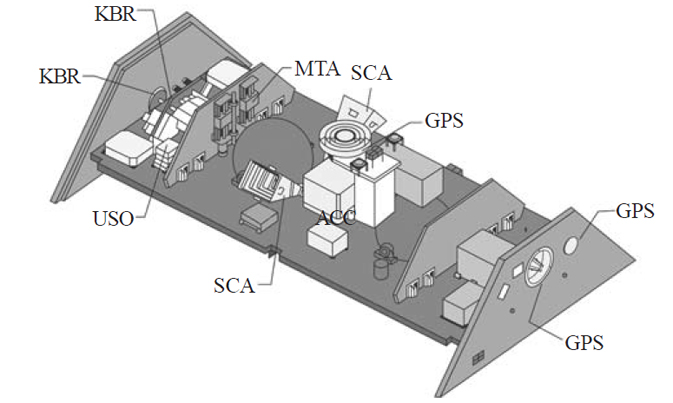
\includegraphics[width=0.7\textwidth]{GRACE_Component.jpg} 
	\caption{GRACE Component} 
	\label{fig:GRACEComponent}
\end{figure}
\begin{itemize}
	\item K-band Ranging System (KBR): Provides precise (within 10 micrometre) measurements of the distance change between the two satellites needed to measure fluctuations in gravity.
	\item Ultra Stable Oscillator (USO): Provides frequency generation for the K-band ranging system.
	\item SuperSTAR Accelorometers (ACC): Precisely measures the non-gravitational accelerations acting on the satellites.
	\item Star Camera Assembly (SCA): Precisely determines the two satellite's orientation by tracking them relative to the position of the stars.
	\item Coarse Earth Sun and Sensor (CES): Provides omnidirectional, reliable, and robust, but fairly coarse, Earth and Sun tracking. Used during initial acquisition and whenever GRACE operates in safe mode.
	\item Center of Mass Trim Assembly (MTA): Precisely measures the offset between the satellite's center of mass and the "acceleration-proof" mass and adjusts center of mass as needed during the flight.
	\item BlackJack GPS Receiver and Instrument Processing Unit (GPS): 	Provides digital signal processing; measures the distance change relative to the GPS satellite constellation.
	\item Globalstar Silicon Solar Cell Arrays (GSA): Covers the outer shell of the spacecraft and generates power.
\end{itemize}
It is shown, that GRACE delivers the highest temporal resolution and is thus able to observe monthly mass variation with a spatial resolution of less than 1000\ut{km}. In \cite{wahr1998time} it was predicted that GRACE would be able to measure these effects with an accuracy of about 2\ut{mm} of water equivalent heights. Though this accuracy has not yet been achieved because of the errors in spherical harmonic coefficients of short-wavelength, it was shown in many publications that the Stokes coefficients from GRACE indeed contain hydrological signals as the monthly solutions from GRACE showed a good agreement with mass variations from hydrological models.
\begin{figure}[htbp]
	\centering
	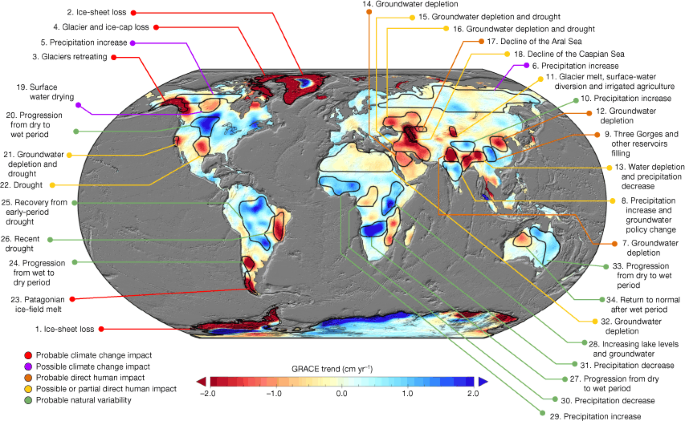
\includegraphics[width=0.89\textwidth]{TWSA} % Datei in "bilder/" bei LaTeX: eps, bei PDFLaTeX: jpg (o.ä.) 
	\caption{global water storage change} 
	\label{fig:TWSA}
\end{figure}
\begin{figure}[ht]
	\centering
	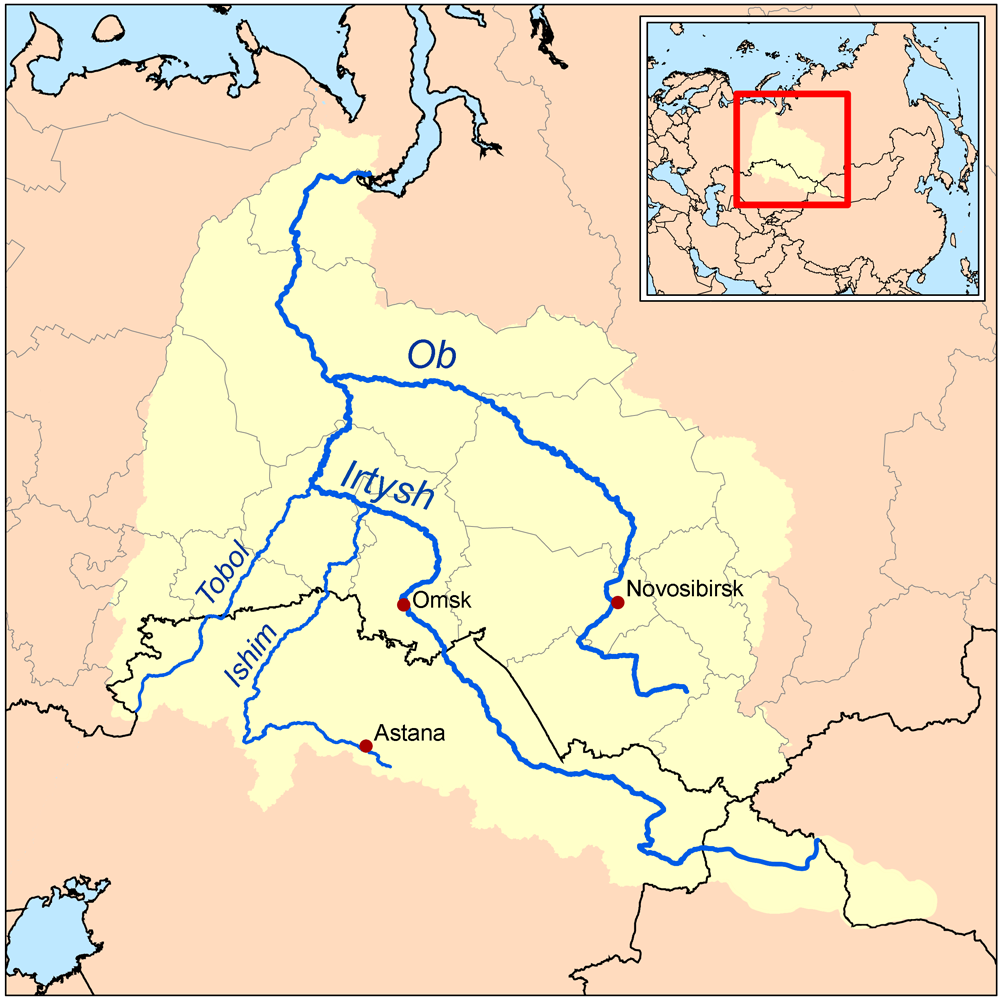
\includegraphics[width=0.9\textwidth]{Obbasin} % Datei in "bilder/" bei LaTeX: eps, bei PDFLaTeX: jpg (o.ä.) 
	\caption{Ob basin} 
	\label{fig:Obbasin}
\end{figure}
\section{Motivation}
In hydrology, most variables are observed in time series, including Total Water Storage Anomaly (TWSA). In the hydrological cycle, this should reflect seasonal behavior and is in long term relatively stable. However, it was shown that since 2002 the TWSA of many big basins has increased (see figure \ref{fig:TWSA}). One important basin of them is Ob basin in west Siberia (see figure \ref{fig:Obbasin}). How did this trend happen is a very interesting topic. Through the analysis of the trend of the time series, it is possible to further understand the changes that have taken place before and future changes can also be predicted based on the stationary analysis.
\section{Objective}
In this thesis, the beginning point of the changing trend is to be found by analyzing the TWSA time series from GRACE data. In order to find the reason of the change, the precipitation, the evatranspiration along with the runoff in the same period from different data center would also be processed and compared with the TWSA. At the end, how was the changes of the TWSA and the reasons for this change would be discussed. 
